\section{Definição de requisitos técnicos e especificações-meta}
\label{sec:definicao_requisitos}

A definição dos requisitos técnicos e das especificações-meta é uma etapa fundamental para garantir que o produto desenvolvido esteja alinhado às necessidades identificadas junto aos usuários e, simultaneamente, seja tecnicamente factível. Nesse processo, busca-se transformar as expectativas e dificuldades relatadas pelos consumidores em características objetivas que possam orientar o desenvolvimento e a avaliação do produto.

A partir da pesquisa realizada com os potenciais usuários, foram identificadas diferentes necessidades relacionadas à jornada de compra no varejo de roupas, especialmente nos aspectos de localização dos produtos, autonomia, pagamento, uso de tecnologia e segurança. Para evitar que essas necessidades sejam traduzidas diretamente em soluções sem uma análise técnica, será utilizado o método \textit{Quality Function Deployment} (QFD). O QFD permite estruturar a chamada ``voz do cliente'' e relacioná-la a requisitos técnicos mensuráveis, possibilitando que as expectativas dos usuários sejam incorporadas ao desenvolvimento do produto.

Além de considerar a importância atribuída pelos clientes, os requisitos técnicos devem ser avaliados quanto à sua factibilidade. Como o presente projeto será desenvolvido em escala de protótipo, as especificações devem ser compatíveis com os recursos financeiros, tecnológicos e materiais disponíveis para a equipe. Dessa forma, o objetivo não é estabelecer requisitos para uma solução industrial definitiva, mas definir metas que permitam verificar se o conceito proposto é capaz de solucionar as principais dores identificadas na pesquisa.

\subsection{Necessidades dos usuários}
\label{subsec:necessidades_usuarios}

A análise das respostas obtidas no questionário permitiu identificar diferentes padrões de comportamento entre os consumidores. Os resultados foram posteriormente organizados nos quatro perfis identificados pela equipe: Cliente Popular com menor autonomia, Consumidor orientado à rapidez, Cliente Premium orientada à conveniência e Compradora para filhos. Os três primeiros grupos concentram a maior parcela da amostra.

Apesar das diferenças entre os grupos, algumas necessidades aparecem de maneira transversal. Um dos principais pontos identificados foi a dificuldade relacionada à \textbf{disponibilidade e localização dos produtos}. Embora a maior parte dos respondentes tenha se mantido neutra quanto à facilidade de encontrar produtos, apenas uma pequena parcela declarou saber previamente se determinado produto estaria disponível na loja. Além disso, 87 respondentes afirmaram que às vezes já saíram de uma loja sem realizar a compra por não encontrar o produto procurado, enquanto outros 18 relataram que isso ocorre frequentemente. Esse resultado indica uma oportunidade relevante relacionada à visibilidade da disponibilidade dos produtos.

Outra necessidade identificada está relacionada à \textbf{agilidade no processo de pagamento}. Dos respondentes, 47 concordaram ou concordaram totalmente que o tempo necessário para pagar é maior do que gostariam. Além disso, 51 respondentes discordaram da afirmação de que o processo de pagamento é simples e rápido, enquanto 44 afirmaram que às vezes já desistiram de uma compra em razão da fila no caixa. Dessa forma, a redução do tempo e da fricção durante o pagamento constitui uma das necessidades centrais para o desenvolvimento da solução.

A \textbf{possibilidade de realizar o pagamento com maior autonomia} também se apresenta como uma necessidade relevante. Embora exista uma parcela significativa de consumidores que ainda valoriza a participação do vendedor, 44 respondentes concordaram ou concordaram totalmente que preferem pagar sozinhos quando isso é possível. Ao mesmo tempo, 75 respondentes discordaram ou discordaram totalmente da afirmação de que preferem escolher os produtos sem auxílio de um vendedor. Isso demonstra que a autonomia não deve necessariamente substituir o atendimento humano em toda a jornada, mas pode ser particularmente relevante em etapas específicas, como o pagamento.

A \textbf{facilidade de utilização da tecnologia} constitui outra necessidade importante. A pesquisa mostrou que os consumidores apresentam níveis diferentes de familiaridade com soluções de autoatendimento. Embora 67 respondentes tenham concordado ou concordado totalmente que já utilizaram algum tipo de autoatendimento sem problemas, 26 discordaram ou discordaram totalmente dessa afirmação. Dessa forma, a solução deve apresentar uma interação simples e intuitiva, evitando que a adoção da tecnologia se transforme em uma nova fonte de dificuldade, especialmente para o perfil de Cliente Popular com menor autonomia.

Também foi identificada a necessidade de \textbf{confiança no pagamento realizado pelo celular}. Embora 41 respondentes tenham concordado ou concordado totalmente que confiam em realizar um pagamento pelo celular sem falar com um funcionário, 40 apresentaram algum grau de discordância. Esse resultado indica que a solução deve fornecer informações claras sobre a confirmação da transação e apresentar mecanismos que transmitam segurança ao usuário.

A \textbf{redução das etapas de verificação na saída da loja} representa outra necessidade potencial. A maioria dos respondentes declarou sentir-se segura ao sair da loja com um produto comprado, porém a aceitação de um processo que eliminasse a checagem manual foi mais dividida. Apenas 33 respondentes concordaram ou concordaram totalmente que confiariam em sair da loja sem essa verificação, enquanto 53 discordaram ou discordaram totalmente. Portanto, embora a eliminação da checagem possa contribuir para uma jornada mais rápida, ela deve estar associada a uma confirmação clara e confiável do pagamento.

A \textbf{facilidade para encontrar tamanho e cor adequados} também foi identificada como uma necessidade. A maioria dos respondentes permaneceu neutra quanto à facilidade de encontrar o tamanho ou a cor desejados, enquanto 15 demonstraram algum grau de discordância. Embora esse resultado seja menos expressivo do que o observado para a disponibilidade dos produtos, essa necessidade apresenta especial relevância para perfis como a Compradora para filhos, para os quais tamanho e disponibilidade podem representar dificuldades adicionais.

Por fim, destaca-se a necessidade de \textbf{manter a possibilidade de atendimento humano quando necessário}. A pesquisa mostrou que 56 respondentes concordaram ou concordaram totalmente que a ausência de um vendedor prejudicaria sua experiência de compra. Esse resultado é particularmente importante para a definição do produto, pois indica que a solução não deve pressupor que todos os consumidores desejam uma jornada completamente autônoma. A tecnologia deve, portanto, reduzir etapas desnecessárias sem eliminar o suporte humano nos momentos em que ele é valorizado.

Com base nesses resultados, foram selecionadas oito necessidades prioritárias para orientar o desenvolvimento do produto:

\begin{enumerate}
\item facilidade para localizar os produtos desejados;
\item maior visibilidade sobre a disponibilidade dos produtos;
\item redução do tempo necessário para realizar o pagamento;
\item possibilidade de realizar o pagamento com autonomia;
\item facilidade e intuitividade na utilização da tecnologia;
\item segurança e confiança no pagamento realizado pelo celular;
\item redução da necessidade de verificações manuais na saída;
\item possibilidade de receber atendimento humano quando necessário.
\end{enumerate}

Essas necessidades constituem a ``voz do cliente'' que será posteriormente traduzida em requisitos técnicos por meio do QFD. A seleção também considera os diferentes perfis encontrados na pesquisa, buscando evitar que o produto seja desenvolvido exclusivamente para o consumidor que apresenta maior familiaridade com tecnologia ou maior preferência por autonomia.

\subsection{Requisitos Técnicos}
\label{subsec:requisitos_tecnicos}

A partir das necessidades identificadas na pesquisa, foram definidos requisitos técnicos que permitem medir objetivamente a capacidade da solução de atender às principais dores dos usuários. Como o produto desenvolvido é composto pela integração entre uma tag física com tecnologia RFID e um aplicativo, os requisitos contemplam tanto o desempenho da tag quanto a interação do usuário com o aplicativo e a comunicação entre os diferentes componentes do sistema.

Os requisitos foram definidos de forma a representar resultados percebidos pelo cliente, e não apenas características isoladas dos componentes. Dessa maneira, aspectos como rapidez, facilidade de uso, confiabilidade e autonomia podem ser avaliados por meio de indicadores objetivos durante os testes do protótipo. As especificações-meta apresentadas nesta seção representam objetivos de desempenho para o protótipo e poderão ser refinadas conforme os resultados das etapas de desenvolvimento e testes.


\paragraph{Tempo para localização do produto}
\label{par:tempo_localizacao_produto}

Além de localizar corretamente o produto, a solução deve reduzir o esforço e o tempo necessário para encontrá-lo. Esse requisito será medido pelo intervalo entre a solicitação do produto pelo usuário no aplicativo e a indicação de sua localização. A especificação-meta é que o sistema apresente a informação necessária para localizar o produto em até \textbf{10 segundos} após a solicitação.


\paragraph{Tempo total para conclusão do pagamento}
\label{par:tempo_total_pagamento}

Esse requisito mede diretamente a capacidade da solução de reduzir o tempo necessário para concluir a compra. Será medido pelo intervalo entre o início do processo de pagamento no aplicativo e a apresentação da confirmação da transação. A especificação-meta é que o processo seja concluído em até \textbf{60 segundos}, desconsiderando atrasos externos provocados por instituições financeiras ou serviços de terceiros.



\paragraph{Taxa de conclusão correta do fluxo no aplicativo}
\label{par:taxa_fluxo_aplicativo}

Esse requisito mede a facilidade de utilização e a intuitividade da interface. Será calculado pela proporção de usuários que conseguem completar corretamente o fluxo principal sem erros e sem receber instruções adicionais da equipe. A especificação-meta é atingir pelo menos 

\paragraph{Tempo para identificação da peça por RFID}
\label{par:tempo_identificacao_tag}

Esse requisito mede a rapidez com que a tag é reconhecida pelo sistema após a aproximação ao dispositivo de leitura. Será medido pelo intervalo entre a aproximação da tag e a identificação correta da peça pelo aplicativo. A especificação-meta é que a identificação ocorra em até \textbf{2 segundos}.

\paragraph{Taxa de leitura correta da tag}
\label{par:taxa_leitura_tag}

Esse requisito mede a confiabilidade da interação entre a tag RFID e o aplicativo. Será calculado pela proporção de tentativas em que a peça é corretamente identificada em relação ao total de tentativas realizadas. A especificação-meta é atingir pelo menos 

\paragraph{Taxa de confirmação correta do pagamento}
\label{par:taxa_confirmacao_pagamento}

Esse requisito mede a confiabilidade das informações apresentadas ao consumidor sobre o estado da transação. Será calculado pela proporção de operações em que o aplicativo informa corretamente ao usuário se o pagamento foi ou não confirmado. A especificação-meta é atingir 
 

\paragraph{Tempo entre confirmação do pagamento e liberação da tag}
\label{par:tempo_liberacao_tag}

Esse requisito mede a rapidez com que a solução responde à confirmação do pagamento, permitindo que o consumidor retire a peça sem necessidade de intervenção de um funcionário. Será medido pelo intervalo entre a confirmação da transação e o acionamento do mecanismo de liberação da tag. A especificação-meta é de, no máximo, \textbf{2 segundos}.


\vspace{10mm}


Em conjunto, esses requisitos permitem avaliar a capacidade da tag e do aplicativo de responder às principais necessidades identificadas na pesquisa. Os primeiros requisitos estão relacionados à localização e à disponibilidade dos produtos, que representam as dores mais relevantes identificadas pelos usuários. Em seguida, são contemplados aspectos de rapidez e autonomia no pagamento, facilidade de utilização da tecnologia e segurança da transação. Por fim, são considerados mecanismos destinados a reduzir a necessidade de verificações e intervenções manuais, sem eliminar a possibilidade de atendimento humano quando este for necessário.



Dessa forma, os requisitos técnicos estabelecidos podem ser utilizados como base para a construção da matriz do QFD, relacionando cada necessidade dos usuários às características técnicas que terão maior influência sobre sua satisfação. A avaliação conjunta dessas relações permitirá priorizar os requisitos de maior impacto para o desempenho percebido do produto.


\subsection{QFD: Quality Function Deployment}
\label{subsec:QFD}


Após a identificação das principais necessidades dos usuários, é necessário traduzi-las em características técnicas que possam orientar o desenvolvimento e permitir a avaliação objetiva do produto. Para isso, será utilizado o método \textit{Quality Function Deployment} (QFD), que permite relacionar sistematicamente a voz do cliente aos requisitos técnicos do produto.

No contexto deste projeto, o QFD será utilizado para estabelecer a relação entre os \textbf{requisitos dos clientes}, identificados a partir da pesquisa realizada com os consumidores, e os \textbf{requisitos técnicos} associados à tag RFID e ao aplicativo. Dessa forma, será possível identificar quais características técnicas possuem maior influência sobre a satisfação das necessidades dos usuários e, consequentemente, devem receber maior atenção durante o desenvolvimento do protótipo.

A utilização do QFD também permite considerar simultaneamente a importância atribuída pelos clientes a cada necessidade e a intensidade da relação entre essa necessidade e cada requisito técnico. Assim, o método contribui para priorizar os aspectos técnicos do produto de maneira alinhada à percepção de valor dos usuários, reduzindo o risco de direcionar os esforços de desenvolvimento para características que possuem menor impacto sobre as necessidades identificadas.

\begin{figure}[H]
    \centering
    \caption{Casa da Qualidade}
    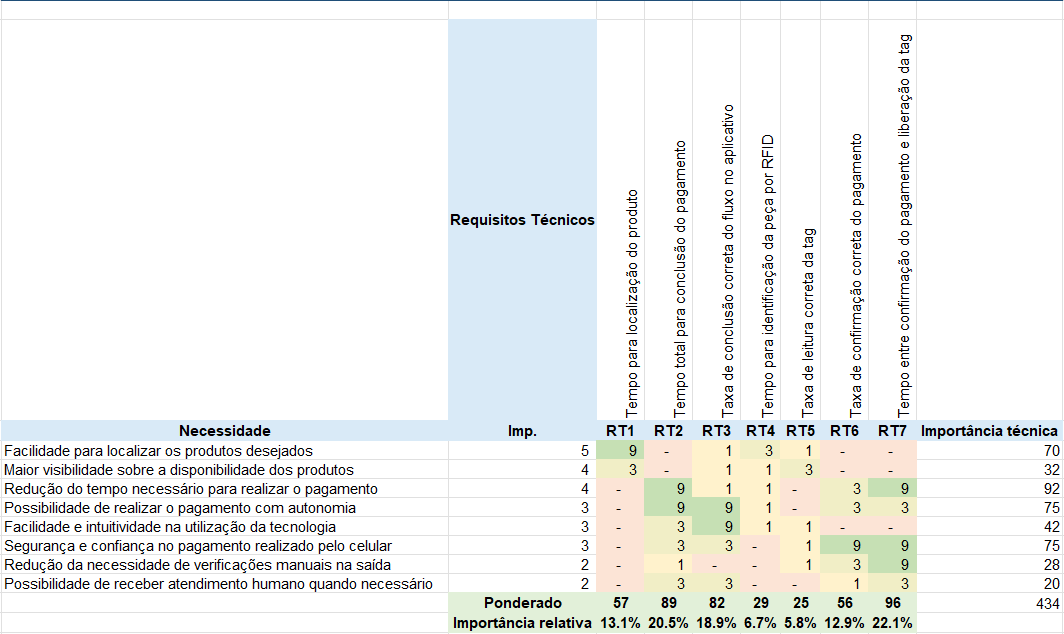
\includegraphics[width=0.9\textwidth]{imagens/definicao dos requisitos/fig01-casa-qualidade-qfd.png}
    \label{fig:casa-qualidade}
    \source{Autoria Própria}
\end{figure}

\begin{figure}[H]
    \centering
    \caption{Teto de correlações}
    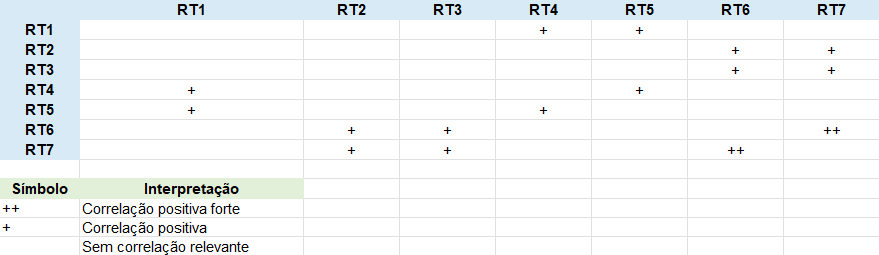
\includegraphics[width=0.9\textwidth]{imagens/definicao dos requisitos/fig02-matriz-correlacao-rt.png}
    \label{fig:teto-correlacoes}
    \source{Autoria Própria}
\end{figure}


A Matriz de Relacionamentos do QFD permite avaliar a intensidade da relação entre cada necessidade identificada junto aos usuários e os requisitos técnicos definidos para o produto. Para essa análise, foram consideradas as relações forte, moderada e fraca, representadas, respectivamente, pelos valores 9, 3 e 1, enquanto a ausência de relação foi representada por 0. A importância técnica de cada requisito foi então obtida considerando a importância atribuída às necessidades pelos clientes e a intensidade de suas respectivas relações.

Os resultados mostram que os requisitos técnicos não apresentam a mesma relevância para o atendimento das necessidades dos usuários. O requisito de maior importância técnica foi o \textbf{tempo entre a confirmação do pagamento e a liberação da tag}, responsável por aproximadamente \textbf{22,1\% da importância técnica total}. Sua elevada importância está associada principalmente às necessidades de redução do tempo necessário para realizar o pagamento, segurança e confiança no pagamento realizado pelo celular e redução da necessidade de verificações manuais na saída. Isso indica que a resposta rápida da tag após a confirmação do pagamento constitui um dos principais pontos técnicos da solução.

O segundo requisito mais relevante foi o \textbf{tempo total para conclusão do pagamento}, com aproximadamente \textbf{20,5\% da importância técnica total}. Esse resultado está diretamente relacionado à necessidade de tornar o processo de pagamento mais rápido e também contribui para a possibilidade de realização da compra com maior autonomia. Dessa forma, o desempenho temporal da solução constitui um fator central para o valor percebido pelo usuário.

Em seguida, a \textbf{taxa de conclusão correta do fluxo no aplicativo} apresentou aproximadamente \textbf{18,9\% da importância técnica total}. Esse requisito possui forte relação com a possibilidade de realizar o pagamento com autonomia e com a facilidade e intuitividade na utilização da tecnologia. O resultado reforça que não é suficiente que o sistema seja funcional, sendo necessário que o usuário consiga completar o processo corretamente por meio do aplicativo.

O \textbf{tempo para localização do produto} apresentou aproximadamente \textbf{13,1\% da importância técnica total}. Apesar de possuir uma importância técnica inferior aos três requisitos anteriores, esse resultado é particularmente relevante devido à elevada importância atribuída à facilidade para localizar os produtos desejados, que foi a necessidade de maior importância entre os clientes. A relação demonstra que a capacidade do sistema de reduzir o tempo necessário para localizar uma peça contribui diretamente para o atendimento dessa dor.

A \textbf{taxa de confirmação correta do pagamento} apresentou aproximadamente \textbf{12,9\% da importância técnica total}. Sua importância está concentrada principalmente na necessidade de segurança e confiança no pagamento realizado pelo celular, além de contribuir para a redução das verificações manuais na saída. Portanto, a correta comunicação do estado da transação representa um requisito importante para gerar confiança no sistema.

A \textbf{taxa de leitura correta da tag} apresentou aproximadamente \textbf{5,8\% da importância técnica total}, enquanto o \textbf{tempo para identificação da peça por RFID} apresentou aproximadamente \textbf{6,7\%}. Embora esses requisitos apresentem menor importância relativa, eles constituem a base tecnológica necessária para o funcionamento da solução. Uma leitura lenta ou incorreta da tag pode comprometer etapas posteriores do processo e, consequentemente, prejudicar a experiência do usuário.

A análise da matriz evidencia, portanto, que os requisitos técnicos de maior prioridade estão concentrados principalmente em três dimensões: \textbf{rapidez do processo}, \textbf{autonomia do usuário} e \textbf{confiabilidade da transação}. Em conjunto, os três requisitos de maior importância técnica correspondem a aproximadamente \textbf{61,6\% da importância técnica total}, demonstrando que o desenvolvimento deve priorizar uma experiência rápida, simples e confiável.

Também é possível observar que a necessidade de \textbf{facilidade para localizar os produtos desejados}, embora seja a necessidade de maior importância atribuída pelos clientes, não resulta necessariamente no requisito técnico de maior importância. Isso ocorre porque uma mesma necessidade pode ser atendida por diferentes características técnicas e porque os pesos do QFD consideram simultaneamente a importância da necessidade e a força de suas relações com os requisitos. Essa característica evidencia a utilidade do método para transformar a voz do cliente em prioridades concretas de desenvolvimento.

Dessa forma, a Matriz de Relacionamentos indica que o protótipo deve concentrar seus esforços principalmente na redução do tempo de pagamento, na correta execução do fluxo no aplicativo, na rapidez da liberação da tag após a confirmação da transação e na confiabilidade das interações entre a tag e o sistema. Esses resultados servirão como base para a definição das especificações-meta e para a priorização das atividades de desenvolvimento e testes do produto.
